\section{REINFORCE}
\begin{frame}{}
    \LARGE Reinforcement Learning: \textbf{REINFORCE}
\end{frame}

\begin{frame}{REINFORCE}
\begin{itemize}
    \setlength{\itemsep}{1em}
    \item REINFORCE is an elegant algorithm for maximizing the expected return.
    \item Intuition: trial and error.
    \item Sample a trajectory $\tau$. If you get a high reward, try to make it more likely; if you get a low reward, try to make it less likely.
    \item A trajectory is a sequence of states, actions, and rewards: $\tau = (s_0, a_0, r_0, s_1, a_1, \cdots)$.
\end{itemize}
\end{frame}

\begin{frame}{REINFORCE}
\begin{itemize}
    \item Expected reward:
        \begin{equation*}
        \begin{split}
            \mathcal{J}(\theta) & = \mathbb{E}_{\tau \sim p(\tau;\theta)}\left[ r(\tau) \right] \\
            & = \int_\tau r(\tau) p(\tau;\theta) d\tau 
        \end{split}
        \end{equation*}
    \pause
    \item Now let’s differentiate this:
        $$
        \nabla_\theta \mathcal{J}(\theta) = \int_\tau r(\tau) \nabla_\theta p(\tau;\theta) d\tau
        $$
        $$
        \text{where} \quad p(\tau;\theta) = \prod_{t \geq 0} p(s_{t+1}|s_t, a_t) \pi_\theta(a_t|s_t)
        $$
    \pause
    \item But this is \textbf{intractable!}
\end{itemize}
\end{frame}

\begin{frame}{REINFORCE}
\begin{itemize}
    \item However, we can use a useful trick:
    \begin{equation*}
    \begin{split}
        \nabla_\theta p(\tau;\theta) & = p(\tau;\theta) \frac{\nabla_\theta p(\tau;\theta)}{p(\tau;\theta)} \\
        & = p(\tau;\theta) \nabla_\theta \log p(\tau;\theta)
    \end{split}
    \end{equation*}
    \pause
    \item Now, if we substitute this back:
    \begin{equation*}
    \begin{split}
        \nabla_\theta \mathcal{J}(\theta) & = \int_\tau \left( r(\tau) \nabla_\theta \log p(\tau;\theta) \right) p(\tau;\theta) d\tau \\
        & = \mathbb{E}_{\tau \sim p(\tau;\theta)}\left[ r(\tau) \nabla_\theta \log p(\tau;\theta) \right]
    \end{split}
    \end{equation*}
    \item We can estimate this with Monte Carlo sampling.
\end{itemize}
\end{frame}

\begin{frame}{REINFORCE}
\begin{itemize}
    \item Recall,
    $$
    p(\tau;\theta) = \prod_{t \geq 0} p(s_{t+1}|s_t, a_t) \pi_\theta(a_t|s_t)
    $$
    \pause
    \item Thus,
    $$
    \log p(\tau;\theta) = \sum_{t \geq 0} \log p(s_{t+1}|s_t, a_t) + \log \pi_\theta(a_t|s_t)
    $$
    \pause
    \item When differentiating:
    $$
    \nabla_\theta \log p(\tau;\theta) = \sum_{t \geq 0} \nabla_\theta \log \pi_\theta(a_t|s_t)
    $$
    \pause
    \item It doesn’t depend on the transition probabilities!
\end{itemize}
\end{frame}

\begin{frame}{REINFORCE}
\begin{itemize}
    \item Therefore, when sampling a trajectory $\tau$, we can estimate $\nabla_\theta \mathcal{J}(\theta)$ as:
    $$
    \nabla_\theta \mathcal{J}(\theta) \approx \sum_{t \geq 0} r(\tau) \nabla_\theta \log \pi_\theta(a_t|s_t)
    $$
    \pause
    \item Interpretation:
    \begin{itemize}
        \item If $r(\tau)$ is high, increase the probabilities of the actions taken.
        \item If $r(\tau)$ is low, decrease the probabilities of the actions taken.
    \end{itemize}
    \pause
    \item It might seem simplistic to say that if a trajectory is good, then all its actions were good. But in expectation, it averages out!
\end{itemize}
\end{frame}

\begin{frame}{REINFORCE}
    \begin{figure}
        \centering
        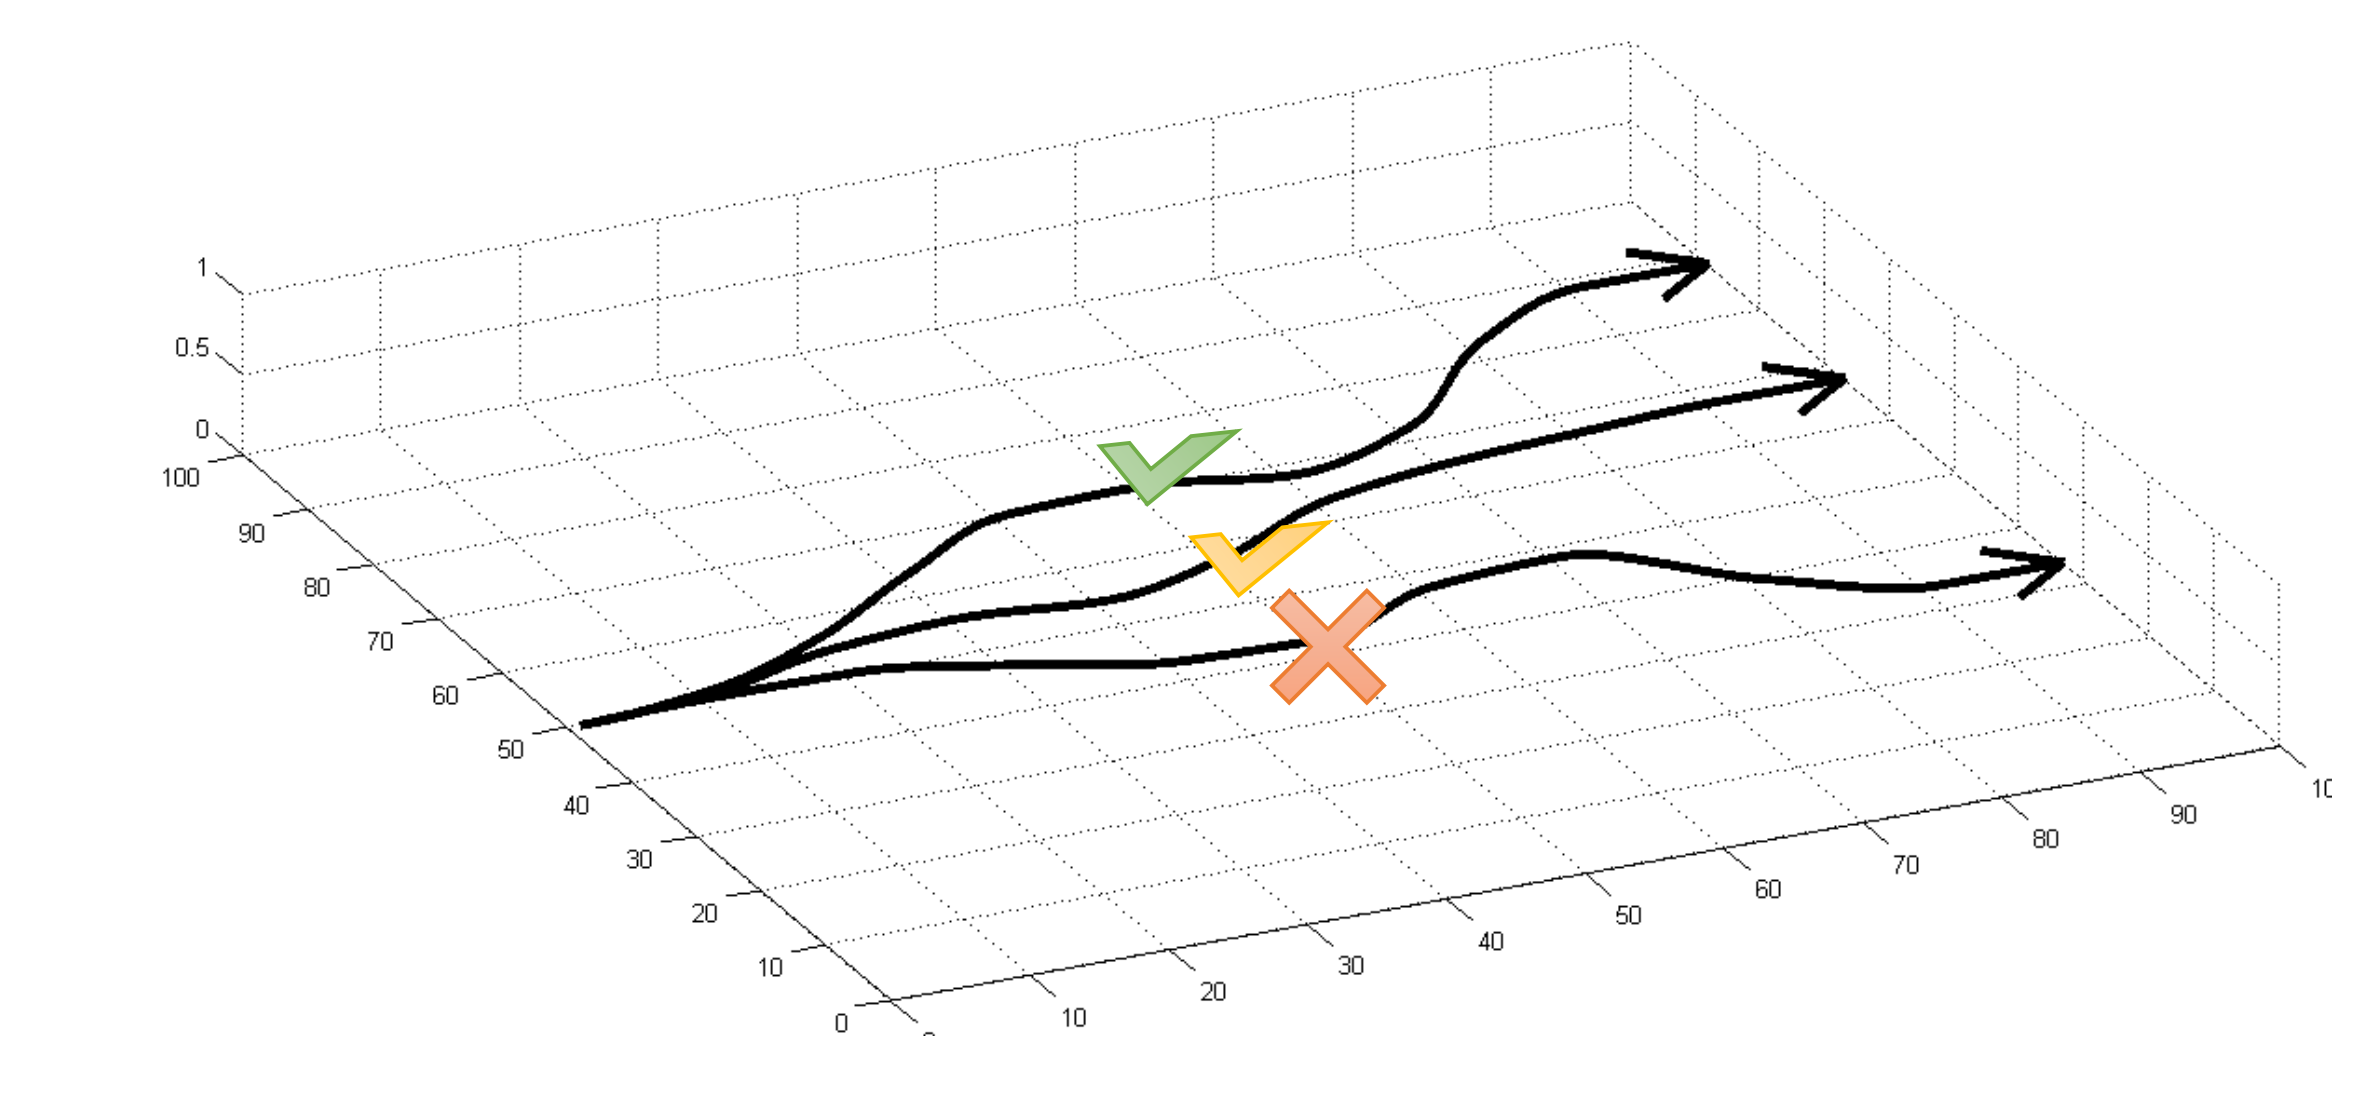
\includegraphics[width=\textwidth,height=0.9\textheight,keepaspectratio]{images/policygrad+reinforce+actor/reinforce.png}
    \end{figure}
\end{frame}

\begin{frame}{REINFORCE Cycle}
    \begin{figure}
        \centering
        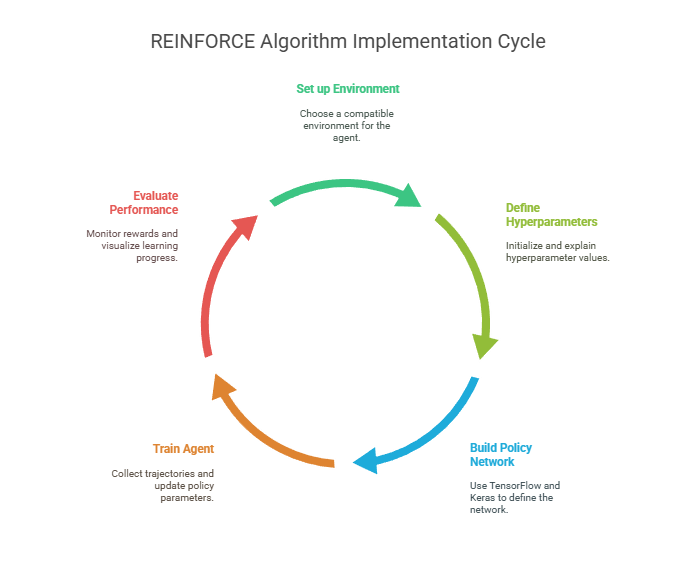
\includegraphics[width=\textwidth,height=0.92\textheight,keepaspectratio]{images/policygrad+reinforce+actor/reinforce_cycle.png}
    \end{figure}
\end{frame}